\chapter{Аналитическая часть}
В данном разделе рассмотрена информация, касающаяся основ конвейерной обработки данных.

\section{Разреженный строчный формат матрицы}

Во многих областях человеческой деятельности информацию
часто представляют в форме матриц. Матрица --- это регулярный
числовой массив. Разреженная  матрица --- матрица, в которой большинство элементов равны нулю.

Разреженный строчный формат (сокр. РСФ)~\cite{csr} --- это одна из наиболее широко используемых схем хранения разреженных матриц.
Эта схема предъявляет минимальные требования к памяти и в то же
время оказывается очень удобной для нескольких важных операций над разреженными матрицами: сложения, умножения,
перестановок строк и столбцов, транспонирования, решения линейных систем с разреженными матрицами коэффициентов как
прямыми, так и итерационными методами и т. д. 
Значения ненулевых элементов матрицы и соответствующие столбцовые индексы хранятся в этой схеме по строкам в двух массивах; назовем их соответственно $AN$ и $JA$. 
Используется также массив указателей (скажем, $AI$, еще обозначающийся как $NR$), отмечающих позиции массивов $AN$ и $JA$, с которых начинается описание очередной строки. Дополнительная компонента в $AI$ содержит указатель первой свободной позиции в $JA$ и $AN$. 
Пример представления матрицы РСФ на рисунке~\ref{fig:ex-csr}.

\clearpage

\begin{figure}[h]
	\centering
	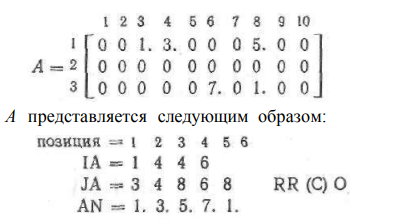
\includegraphics[width=0.85\textwidth]{img/example_csr.png}
	\caption{Пример представления матрицы в РСФ}
	\label{fig:ex-csr}
\end{figure}

В общем случае описание i-й строки $А$ хранится в позициях с $IA(i)$ до $IA(i + 1)$ --- 1 массивов $JA$ и $AN$, за исключением
равенства $IA(i + 1) = IA(i)$, означающего, что r-я строка пуста.
Если матрица $А$ имеет $n$ строк, то $IA$ содержит $n + 1$ позиций. 

\section*{Вывод}
В данном разделе было рассмотрено понятие разреженной матрицы.
